\documentclass[a4paper]{paper}

\usepackage{amsmath}
\usepackage{amsfonts}
\usepackage{amssymb}
\usepackage{tikz}

\usetikzlibrary{shapes,arrows,positioning}

\begin{document}

% Execution tree a statement
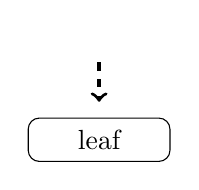
\begin{tikzpicture}[align=center, node distance=0.9cm and -0.6cm]
    \tikzset{
        n/.style        =   { rectangle
                            , rounded corners
                            , text centered
                            , draw=black
                            , minimum width=1.8cm
                            , minimum height=0.55cm
        }
        , arrow/.style  =   { very thick
                            , shorten >= 0.2cm
                            , shorten <= 0.2cm
        }
        , dotted/.style =   { very thick
                            , dashed
                            , shorten >= 0.2cm
                            , shorten <= 0.2cm
        }
    }
    \node(0)                {};
    \node(1)[n, below=of 0] {leaf};

    \draw[dotted,->] (0) -- (1);
\end{tikzpicture}

% Execution tree a simple statement (1)
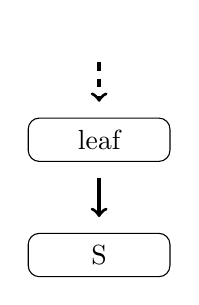
\begin{tikzpicture}[align=center, node distance=0.9cm and -0.6cm]
    \tikzset{
        n/.style        =   { rectangle
                            , rounded corners
                            , text centered
                            , draw=black
                            , minimum width=1.8cm
                            , minimum height=0.55cm
        }
        , arrow/.style  =   { very thick
                            , shorten >= 0.2cm
                            , shorten <= 0.2cm
        }
        , dotted/.style =   {  very thick
                            , dashed
                            , shorten >= 0.2cm
                            , shorten <= 0.2cm
        }
    }
    \node(0)                {};
    \node(1)[n, below=of 0] {leaf};
    \node(2)[n, below=of 1] {S};

    \draw[dotted,->] (0) -- (1);
    \draw[arrow,->]  (1) -- (2);
\end{tikzpicture}

% Execution tree an if-then-else statement (1)
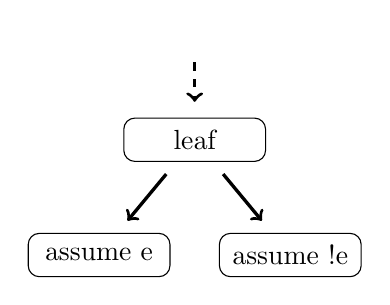
\begin{tikzpicture}[align=center, node distance=0.9cm and -0.6cm]
    \tikzset{
        n/.style        =   { rectangle
                            , rounded corners
                            , text centered
                            , draw=black
                            , minimum width=1.8cm
                            , minimum height=0.55cm
        }
        , arrow/.style  =   { very thick
                            , shorten >= 0.2cm
                            , shorten <= 0.2cm
        }
        , dotted/.style =   {  very thick
                            , dashed
                            , shorten >= 0.2cm
                            , shorten <= 0.2cm
        }
    }
    \node(0)                {};
    \node(1)[n, below=of 0] {leaf};
    \node(2)[n, below left=of 1] {assume e};
    \node(3)[n, below right=of 1] {assume !e};

    \draw[dotted,->] (0) -- (1);
    \draw[arrow,->]  (1) -- (2);
    \draw[arrow,->]  (1) -- (3);
\end{tikzpicture}

% Execution tree an if-then-else statement (2)
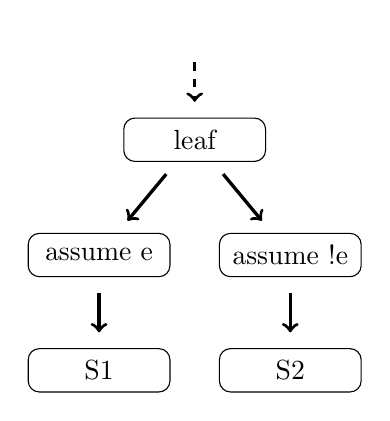
\begin{tikzpicture}[align=center, node distance=0.9cm and -0.6cm]
    \tikzset{
        n/.style        =   { rectangle
                            , rounded corners
                            , text centered
                            , draw=black
                            , minimum width=1.8cm
                            , minimum height=0.55cm
        }
        , arrow/.style  =   { very thick
                            , shorten >= 0.2cm
                            , shorten <= 0.2cm
        }
        , dotted/.style =   {  very thick
                            , dashed
                            , shorten >= 0.2cm
                            , shorten <= 0.2cm
        }
    }
    \node(0)                {};
    \node(1)[n, below=of 0] {leaf};
    \node(2)[n, below left=of 1] {assume e};
    \node(3)[n, below right=of 1] {assume !e};
    \node(4)[n, below=of 2] {S1};
    \node(5)[n, below=of 3] {S2};

    \draw[dotted,->] (0) -- (1);
    \draw[arrow,->]  (1) -- (2);
    \draw[arrow,->]  (1) -- (3);
    \draw[arrow,->]  (2) -- (4);
    \draw[arrow,->]  (3) -- (5);
\end{tikzpicture}

% Execution tree a while loop (1)
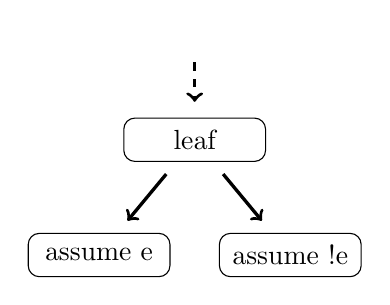
\begin{tikzpicture}[align=center, node distance=0.9cm and -0.6cm]
    \tikzset{
        n/.style        =   { rectangle
                            , rounded corners
                            , text centered
                            , draw=black
                            , minimum width=1.8cm
                            , minimum height=0.55cm
        }
        , arrow/.style  =   { very thick
                            , shorten >= 0.2cm
                            , shorten <= 0.2cm
        }
        , dotted/.style =   { very thick
                            , dashed
                            , shorten >= 0.2cm
                            , shorten <= 0.2cm
        }
    }
    \node(0)                {};
    \node(1)[n, below=of 0] {leaf};
    \node(2)[n, below left=of 1] {assume e};
    \node(3)[n, below right=of 1] {assume !e};

    \draw[dotted,->] (0) -- (1);
    \draw[arrow,->]  (1) -- (2);
    \draw[arrow,->]  (1) -- (3);
\end{tikzpicture}

% Execution tree a while loop (2)
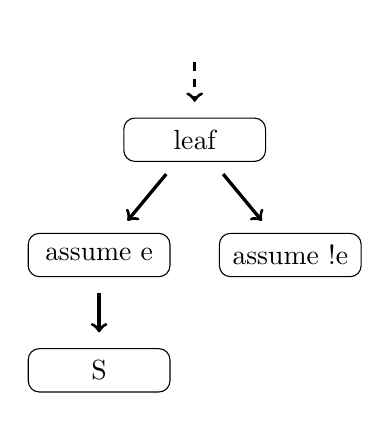
\begin{tikzpicture}[align=center, node distance=0.9cm and -0.6cm]
    \tikzset{
        n/.style        =   { rectangle
                            , rounded corners
                            , text centered
                            , draw=black
                            , minimum width=1.8cm
                            , minimum height=0.55cm
        }
        , arrow/.style  =   { very thick
                            , shorten >= 0.2cm
                            , shorten <= 0.2cm
        }
        , dotted/.style =   { very thick
                            , dashed
                            , shorten >= 0.2cm
                            , shorten <= 0.2cm
        }
    }
    \node(0)                {};
    \node(1)[n, below=of 0] {leaf};
    \node(2)[n, below left=of 1] {assume e};
    \node(3)[n, below right=of 1] {assume !e};
    \node(4)[n, below=of 2] {S};

    \draw[dotted,->] (0) -- (1);
    \draw[arrow,->]  (1) -- (2);
    \draw[arrow,->]  (1) -- (3);
    \draw[arrow,->]  (2) -- (4);
\end{tikzpicture}

% Execution tree a while loop (2)
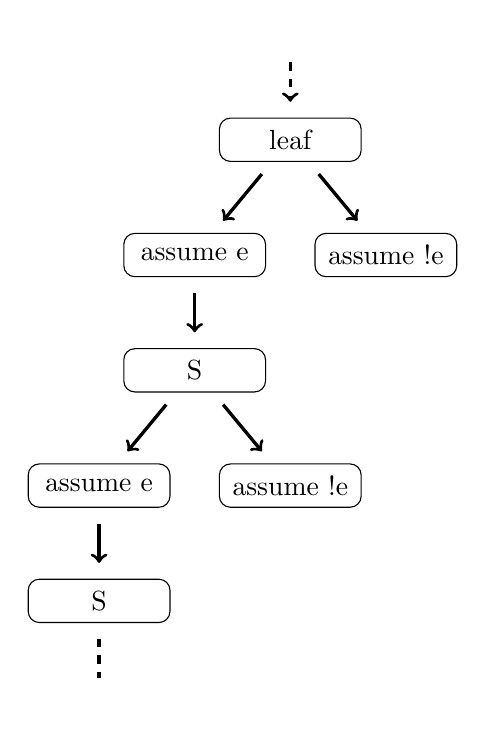
\begin{tikzpicture}[align=center, node distance=0.9cm and -0.6cm]
    \tikzset{
        n/.style        =   { rectangle
                            , rounded corners
                            , text centered
                            , draw=black
                            , minimum width=1.8cm
                            , minimum height=0.55cm
        }
        , arrow/.style  =   { very thick
                            , shorten >= 0.2cm
                            , shorten <= 0.2cm
        }
        , dotted/.style =   { very thick
                            , dashed
                            , shorten >= 0.2cm
                            , shorten <= 0.2cm
        }
    }
    \node(0)                {};
    \node(1)[n, below=of 0] {leaf};
    \node(2)[n, below left=of 1] {assume e};
    \node(3)[n, below right=of 1] {assume !e};
    \node(4)[n, below=of 2] {S};
    \node(5)[n, below left=of 4] {assume e};
    \node(6)[n, below right=of 4] {assume !e};
    \node(7)[n, below=of 5] {S};
    \node(8)[below=of 7] {};

    \draw[dotted,->] (0) -- (1);
    \draw[arrow,->]  (1) -- (2);
    \draw[arrow,->]  (1) -- (3);
    \draw[arrow,->]  (2) -- (4);
    \draw[arrow,->]  (4) -- (5);
    \draw[arrow,->]  (4) -- (6);
    \draw[arrow,->]  (5) -- (7);
    \draw[dotted]    (7) -- (8);
\end{tikzpicture}

% Execution tree a simple statement (2)
%\begin{tikzpicture}
%    \node(0)                {};
%    \node(1)[n, below=of 0] {leaf};
%    \node(2)[n, below=of 1] {S};
%
%    \draw[dotted,->] (0) -- (1);
%    \draw[arrow,->]  (1) -- (2);
%\end{tikzpicture}

%\begin{tikzpicture}%[node/.style = {draw=black, thick, elipse}, node distance=1cm]
%    \tikzset{
%        n/.style        =   { rectangle
%                            , rounded corners
%                            , text centered
%                            , draw=black
%                            }
%        , arrow/.style  =   { very thick
%                            , shorten >= 0.2cm
%                            , shorten <= 0.2cm
%                            }
%    }
%    \node(1)[n] {int result = 0;};
%    \node(2)[n,below=of 1] {int a = 0, b = 1;};
%    \node(3)[n,below=of 2] {int i = 0;};
%    \node(4)[n,below=of 3] {for (i \textless \enskip n)};
%    \node(5)[n,right=of 2] {result = a + b;};
%    \node(6)[n,below=of 5] {b = a;};
%    \node(7)[n,below=of 6] {a = result;};
%    \node(8)[n,below=of 7] {i++};
%    \node(9)[n,below=of 4] {return result;};
%
%    \draw[arrow,->] (1) -- (2);
%    \draw[arrow,->] (2) -- (3);
%    \draw[arrow,->] (3) -- (4);
%    \draw[arrow,->] (4) -- (5);
%    \draw[arrow,->] (4) -- (9);
%    \draw[arrow,->] (5) -- (6);
%    \draw[arrow,->] (6) -- (7);
%    \draw[arrow,->] (7) -- (8);
%    \draw[arrow,->] (8) -- (4);
%\end{tikzpicture}
\end{document}